\documentclass{article}
\usepackage{style-assessments}

% define macros (/shortcuts)
\newcommand{\follow}[1]{\sim \text{#1}\,}		% shortcut for ~ 'Named dist ' in normal font with space before parameters would go



\begin{document}

\hspace{375pt}Name:

\begin{center}
{\Huge MATH 321: In-Class 7-6}
\end{center}

\bigskip\bigskip

% problem types summary
% 1) two sample t test (two tailed), pooled variances, traditional method and CI
% 2) one sample Prop Z-test (one tailed), p-value method, one-sided CI
% 3) paired t test, traditional and p-value method
% 4) min sample size for proportions
% 5) min sample size for one mean



\begin{enumerate}
    \item Two methods for teaching reading were applied to two randomly selected groups of elementary schoolchildren and then compared on the basis of a reading comprehension test given at the end of the learning period. The sample means and variances computed from the test scores are shown below. Assume scores for both methods are normally distributed with unknown, common variance $\sigma^2$.
    \[\text{Method I}: \hspace{10pt} n_1 = 11, \bar{x}_1 = 64, s^2_1 = 52 \hspace{40pt} \text{Method II}: \hspace{10pt} n_2 = 14, \bar{x}_2 = 69, s^2_2 = 71\]
    \begin{enumerate}% Math stats with apps problem 
        \item Do the data present sufficient evidence to indicate a difference in the mean scores for the populations associated with the two teaching methods? Use $\alpha = 0.10$ and make the conclusion using the ``traditional'' method (RR).\vspace{150pt}
        \item Confirm the result in (a) by constructing a two-sided 90\% confidence interval for $\mu_1 - \mu_2$ and seeing if $D_0 = 0$ is in the interval.\vspace{60pt}% Original addition
    \end{enumerate}
    
    \item According to the Washington Post, nearly 45\% of all Americans are born with brown eyes, although their eyes don't necessarily stay brown. A random sample of 80 adults found 30 with brown eyes.% Math stats with apps problem 10.26
    \begin{enumerate}
        \item Is there sufficient evidence at the $\alpha = 0.05$ level to indicate that the proportion of brown-eyed adults is less from the proportion of Americans who are born with brown eyes? Make the conclusion using the ``p-value'' method.\vspace{130pt}% changed alternative to less than
        \item If $\alpha = 0.01$ instead, would the same conclusion be made? How about $\alpha = 0.10$? Explain.\vspace{20pt}% Original addition
        \item Confirm your conclusion from (b) when $\alpha = 0.10$ by constructing the appropriate one-sided 90\% confidence interval for $p$ and seeing if $p_0 = 0.45$ is in the interval.\vspace{60pt}% Original addition
    \end{enumerate}
    
    \item To test whether a golf ball of brand A is better or worse than Brand B, 9 golfers hit a ball of each brand off the tee and measured the distance. The results for the difference in distances ($A - B$) in yards are shown below. Assume that the paired differences in distance are approximately normally distributed.% Stat inference 8.1-12 (changed wording a bit), but only using part of the data and already calculated the differences for them
    \item[]  With $\alpha = 0.05$, test if there is a difference in average distance between brand A and brand B. Make sure to find the RR and the p-value and state any additional insights in the conclusion.% last parts are original additions
    \begin{figure}[H]
        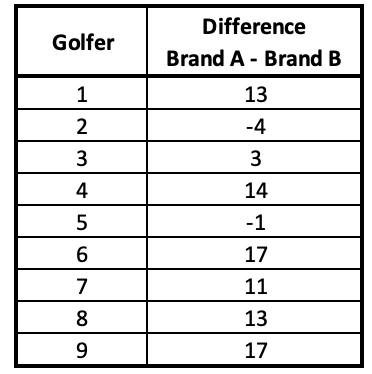
\includegraphics[scale=0.5]{images/data-golf.png}
    \end{figure}\vspace{100pt}
    
    \item Some college professors and students were interested in studying a certain characteristic in Canadian geese and would like to estimate $p$, the proportion of birds with this characteristic.% Stat inference 7.4-8 (changed context a bit)
    \begin{enumerate}
        \item Determine the minimum sample size needed to estimate $p$ within $\epsilon = 0.04$ with 90\% confidence.\vspace{30pt}%Original addition
        \item A previous study took a random sample of 137 Canadian geese and found that 54 had this characteristic. Taking this into account, determine the minimum sample size needed to estimate the unknown $p$ within $\epsilon = 0.04$ with 90\% confidence.\vspace{30pt}% Original question, tweaked a bit
    \end{enumerate}
    
    \item Let $X$ equal the tarsus length for a male grackle. Assume that the distribution of $X \follow{N}(\mu, \sigma^2 = 4.84)$. Find the sample size $n$ that is needed to achieve a maximum error of the estimate of% Stat inference 7.4-1 (added parts)
    \begin{enumerate}
        \item $\epsilon = 0.04$ for a 95\% CI for $\mu$\vspace{40pt}
        \item $\epsilon = 0.08$ for a 85\% CI for $\mu$\vspace{40pt}
    \end{enumerate}
        
\end{enumerate}

\end{document}